% High level idea:
% Introduce timestamped units into the simulator graph, existing models remain implicitly timestamped.

The fundamental assumption made in the previous chapter was that the clocks of
the target cannot change as a function of the simulated behavior of the target
itself. This permits generating a clock-token stream that can runahead of the
rest of the simulator and gives good simulation performance. Lifting this
assumption introduces a potentially performance critical feedback loop into the
emulator: scheduled clocks determine when target state updates occur, but those
updates themselves affect when target clocks are scheduled.
% We illustrate this with a simple example\TODO(clock mux).

Academic work in this domain is lacking. The only hardware-accelerated platform
for studying platforms that can preform DVFS was built by Mantovani et
al.~\cite{DVFSPrototype}. However, that work is essentially a configurable FPGA
prototype: it presupposes a particular target organization~(a grid of tiles
innerconnect with a NoC) and directly directly instantiates FPGA specific
clocking primitives. Using FPGA clocking primitives directly skirts preformance
challenge we outlined above, allowing their system to run fast (100 MHz on a
Virtex 7 FPGA). This makes it an attractive platform to do research on new
DVFS policies, but not generally useful for doing pre-silicon verification or
performance validation of an SoC which does not derive from their input RTL.

For examples of FPGA-based hardware emulation of systems that support dynamic
frequency scaling, one must look to industry. Mentor Veloce and Synopsys ZeBu,
both have support for systems that do this sort of frequency scaling --- how
they support this is propertiary. One 2013 Mentor Graphics patent provides some
insight as to how this may be implemented in Veloce: a compiler detects
``clock-enabling" functions in the target circuit, which are in-essence,
combinational logic functions that permit a clock to be driven to a particular
output node. For instance, the and-gate of a clock gate would be such a
function, controlled by a "clock-enabling singal" the output of the latch. More
complex circuits, like clock multiplexers, can be decomposed into exclusive
sets of these enabling functions. These functions are combined into a single
``clock status" signal which indicate to the emulation clock generator that it
should drive a clock into the sink domain. Many critical details in this system
are intentionally left vague, and context related to emulator clock generation
is omitted.  What appears to be the case is that target behavior governing
clock selection and generation is managed at combinational level, which is a
sensible design decision for generalizing support for a broad range of targets.
It does seem to tightly couple clock generation and to target logic simulation.
One intriguing omission is the lack fine-grained timestamping, which in
conjuction with the observation above, seems to suggest some sort of
centralized control with minimal decoupling acrossing the emulator.

The approach we outline in this chapter is radically different than those
outlined above, in that clock generation and selection circuits are replaced
with indepedent decoupled units that are timestamped. In effect, this subgraph
combined with the hub unit are a conservative PDES, and the resulting simulator
is ETDC.  In our implementation, no FPGA specific clock selection logic beyond
a clock gate, is used, making our implementation portable across different
FPGAs. In also maps well to inherently parallel nature of clock generation and
selection in a SoC. However, this implementation strategy begets its own
challenges however, notably the classic conservative PDES challenge achieving
good performance and avoiding deadlock hinges on finding sufficient lookahead,
which in some cases may not be possible without restricting target behavior.

\section{Context, Goals and Motivation}

To understand how we arrived at our implementation, we need to re-evaluate the
goals we outlined when we designed Golden Gate~(Section~\ref{sec:gg-design-objectives}) given the current capability
of FIRRTL to express clocking primitives, and the machinery available in Golden
Gate to implement these features. These goals were:

\begin{enumerate}
\item \textbf{Maintain FireSim feature completeness.} Just as in the orginal
redesign, it was critical that support for dynamic frequency scaling work in
conjunction with existing bridges and multi-cycle resource optimizations. For
the purposes of getting to a working prototype, we will accept a loss of
simulation FMR. In the long run however, our goal is to support simulating
systems that dynamically change their clocks at the same rate as an equivalent
systems that do not.

\item \textbf{Minimize user modification of ASIC RTL.}
Specifically, we want to avoid extensive changes to the designs module
    hierarchy. The use of a singleton clock bridge in the previous chapter,
    violated this objective. Here, we'll permit replacing ASIC
    clock-generating circuits with inexact models, but we wish to avoid
    centralizing all clock-generation at a single point in the design.

\item \textbf{Provide a mechanism to rigorously verify simulation models.} We
decided to punt on this objective here. Though, as in LI-BDN case, it would be
nice in the future if parts of the simulator could be verified against the
underlying ASIC implementation using a LIME-like flow. In this chapter
we relied on dynamic verification to test additions to our system.

\item \textbf{Enable the use of FireSim as a library for hardware emulation.}
This is closely related to the second point. Clocking and reset structures
remain the single largest point of divergence between ``Chip" configurations and
FireSim configurations of Chipyard SoCs.

\item \textbf{Avoid use of FPGA-specific Clocking Primitives.}
In the interest of supporting other FPGAs in the future, and to avoid more of
the placement and DRC challenges associated with using those devices,
we wanted a design that used conventional logic and interconnect
resources where possible.
\end{enumerate}

Contextually, an important reality to grasp is that native support for clocking
structures in FIRRTL is nascent, and designers tend to use black-box verilog to
describe structures that act on clocks~(these typically have process-specific
implementations that will be used in physical design). Building a compiler
capable of analyzing a hybrid FIRRTL-verilog netlist without designer help was
going to be challenging, as so is left to future work.

%Here we skirt this issue by relying on wholesale
%replacement of these structures, as a stepping stone towards automatic
%generation of models for these circuits in the future.

\section{Designs We Considered}

%For many of the same reasons descrbed the previous chapter, an
%FPGA-prototyping-based approaches like the one described by Mantovani et
%al.~\cite{DVFSPrototype} was off the table.

To resuse most of our work in building out static multiclock support, we
initially tried to frame dynamic clock domain support as solving the smaller
problem of reconstituting the clock-token stream. The most straightforward way
of doing so is to a provide a means for users to specify that certain clocks
have dynamic behavior on the centralized clock bridge. For these clocks, the
clock bridge would accept a parameters to describe how it derives from other
clock in the system (e.g., it should in effect simulate a clock mux and select
between two other output clocks). Based on this selected behavior new inputs on
the bridge would be exposed and driven by target RTL. This would require the
smallest modification to existing infrastructure: bridge extraction would expose
clock-bridge sunk channels for the control signals, and the hub could be modified
to enqueue output tokens on all timesteps for these channels.

While this would suffice for simulating simple systems, the main problem with this approach is that it forces the
designer to reexpress, in a centralized fashion, how all clocks in a system are
generated. This runs counter to the inherently distributed process of clock generation and distribution in an SoC.
In a simple system, a clock source might feed a centralized PLL with closely coupled output dividers,
which in turn may drive downstream dividers, clock muxes and
ICGs distributed throughout the chip. This simplified model is complicated by I/O
devices which tend to provide their own clock generation schemes that derive from still other off-chip clocks. 
As such, it would be better if information about target clocks could be
captured or inferred at the instantion sites of the ASIC circuits that are
responsible for generating derived clocks instead of forcing the user to
rexpress these properties at the clock bridge.

With this in mind, we set out desiging a system that would transform or replace
ASIC circuits with FPGA-compatible equivalents. As in the previous chapter,
this cannot be achieved simply by substituting a primitive with an FPGA analog,
but instead requires a custom representation of that circuit that timing
accurate and deterministic under variable host timings.

The defining design decision of this project was whether to replace
these clock-generating circuits with independent, decoupled units or whether
the compiler should attempt to centralize them into a single chunk of logic
integrated into the hub. In effect this reduces to a question of distributed
versus centrailized control and local versus global optimization. In the
prototype we describe in this chapter, we opted for a distributed approach.
First, it was a natural extension of the Golden Gate framework. Replacing
modules with decoupled units slots neatly into the existing abstractions and so
reuses much of the existing infrastructure. Second, it made it easier to reason
about correctness of pieces of the target independently. Finally, we would be
remiss to omit mentioning that it seemed like a more unique and interesting
system to study, whereas the converse would look more similar to the Cadence
patent we introduced previously. At the end of this chapter~(Section~\ref{sec:pdes-future-work}) we
circle back and more carefully evaluate this tradeoff.

%If clock generation and switching circuits are going to be replaced with independent units,

Until now, units, with the exception of the hub unit and clock bridge, have
represented SSMs. The SSM abstraction clearly does not apply to circuits whose
inputs and outputs are clocks, often without phase relation to one another.
Here, some timekeeping can no longer remain implicit: the times of each input
must be known with respect to one another. To resolve this, we opted to
introduce explicited timestamping in these channels. This makes our
implementation an ET-DC simulator, akin to an FPGA-hosted conservative PDES. We
describe it detail in the next section.

\section{Initial Implementation}

To summarize, our approach functions by replacing modules
related to clock generation, switching, or gating, or behaviors that are
otherwise asynchronous to a clock, with timestamped units. Strictly speaking,
both timestamped and untimestamped units are logical processes~(LP), in this
chapter we will use LP and timestamped unit~(TU) interchangably. TUs are
extracted and replaced in the same fashion as a bridge or an optimized model,
however, their channels are labelled as \emph{timestamped}. Like any
conventional PDES, TUs send \emph{messages} consisting a 2-tuple consisting of
a data value and a timestamp.  In a similar sense, tokens can be thought of as
implicitly-timestamped messages, however we'll reserve the term messages for
timestamped transmissions and tokens to refer to their untimestamped
analogs.

Under this approach, simulator graphs consist of two halves: an untimestamped
subgraph, which includes all of the optimized models and conventional bridges
described in previous chapters. and a timestamped subraph, which includes the
TUs.  The one exception to this rule is the hub unit, which has both
timestamped and untimestamped  channels and resides in both subgraphs. We show
an example graph in Figure~\ref{fig:gg-graph-pdes}.

\begin{figure}
    \centering
    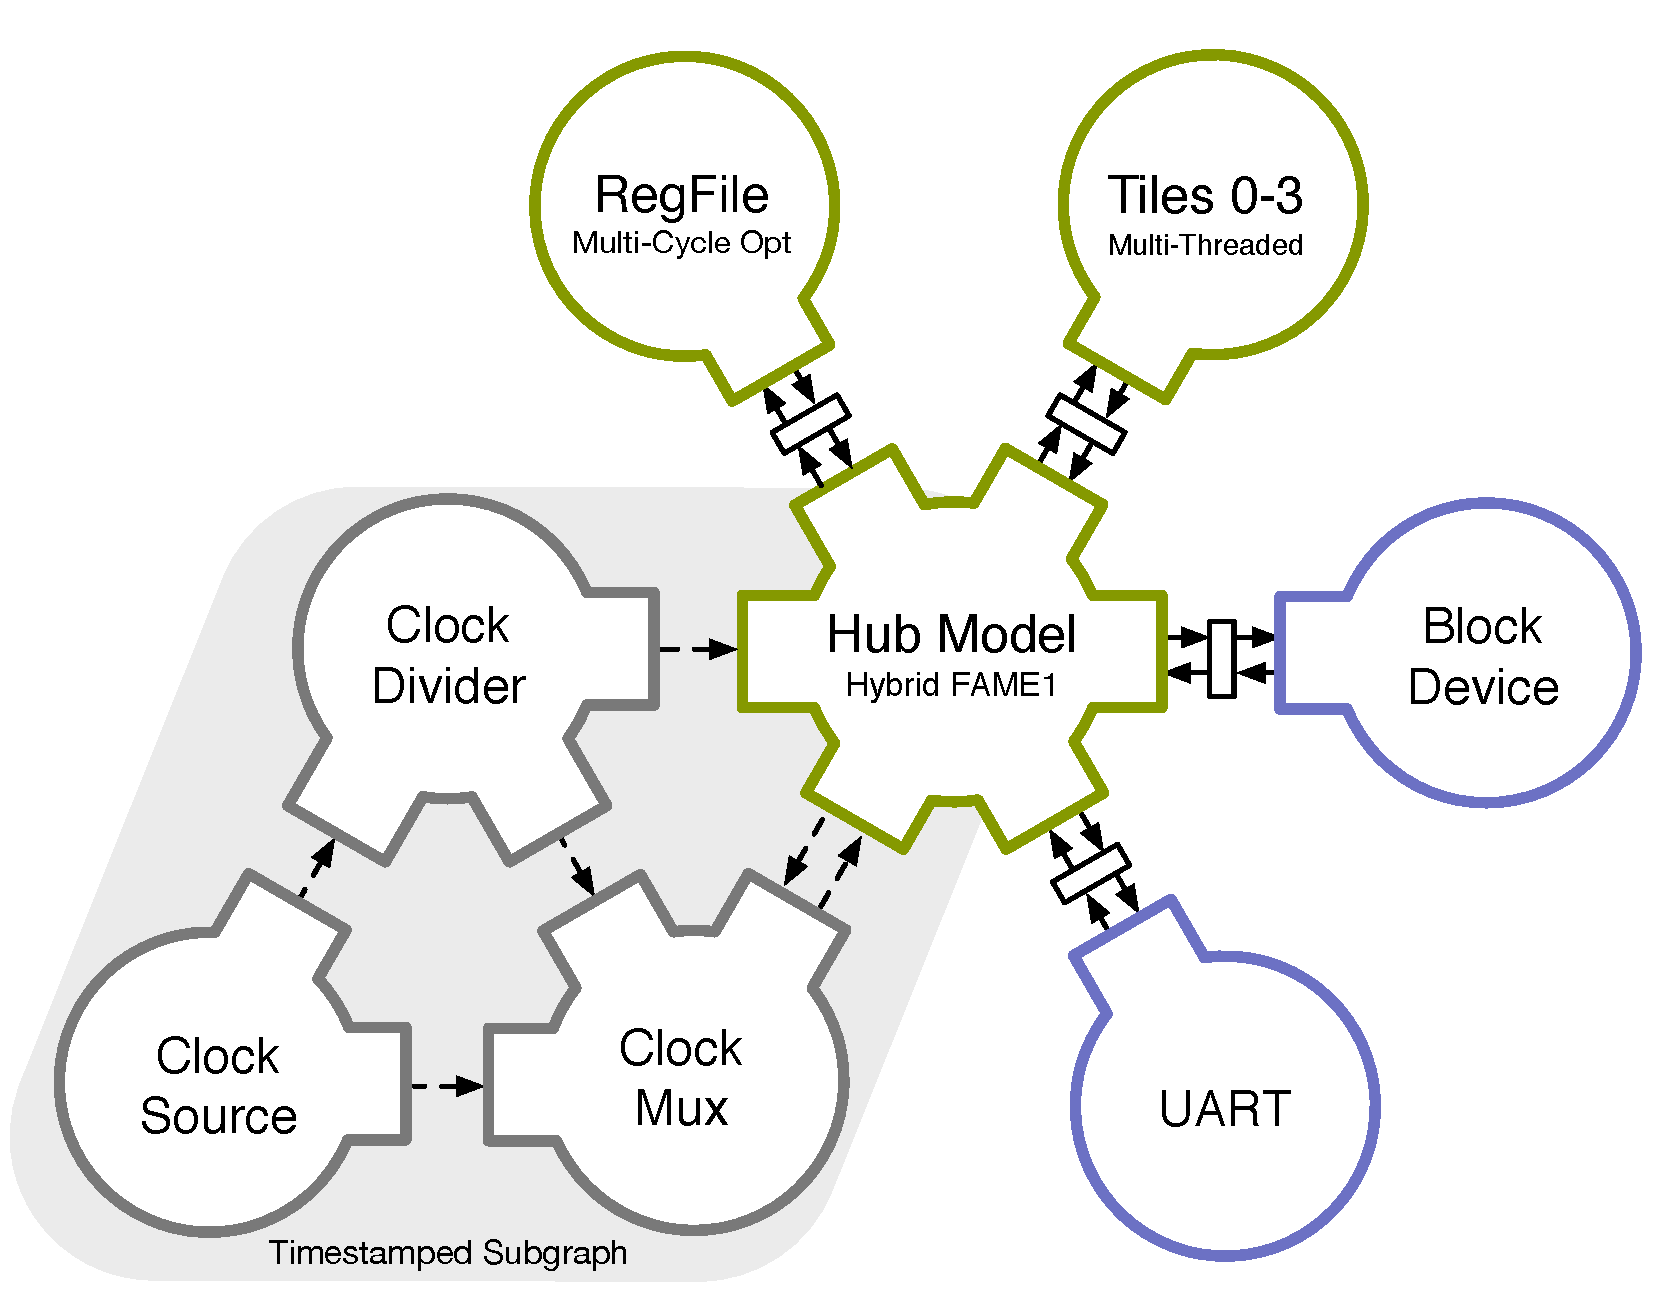
\includegraphics[width=0.99\textwidth]{figures/gg-graph-pdes.pdf}
    % NB: Bounding box of the timestamped subgraph screws up pdf whitespace
    % -c pdes midas-graphics/graffle/midas2-target.graffle figures/gg-graph-pdes.pdf
    \caption{An example simulator graph with a timestamped subgraph
    responsible for modelling clock generation.  Note, the ports represented in
    timestamped models are logical. The clock divider and clock mux both have a
    single output: output messages are duplicated and transmitted to each sink
    over separate channel.}
    \label{fig:gg-graph-pdes}
\end{figure}

For this approach to have acceptable performance, we needed to permit TUs to
send messages directly to one another, instead of forcing these transmissions
to propagate through the hub.  To do so, we introduced a compiler optimization
that removes passthrough connectivity in the hub, permitting two units
(timestamped or untimestamped) to drive each other directly. As a result,
simulator graphs are no longer guaranteed have a star topology (this is
viisible in Figure~\ref{fig:gg-graph-pdes}).  While essential for the prototype
described here, this optimization also improves FMR in designs described in
previous chapter when multiple optimizations are enabled. We expand on this
optimization and other compiler modifications in Section~\ref{sec:pdes-compiler-modifications}

Since there is no longer a clock token stream, we modified the hub unit to
schedule across multiple timestamped inputs. Timestamped inputs can be either
clock-type or data-type~(used for modeling asynchronous resets), these differ
in how they are presented to target RTL. The hub unit explicitly tracks target
time, which it uses to populate the timestamps of output messages as it advances.
We expand on the hub-unit modifications in Section~\ref{sec:pdes-hub-modifications}.

TUs units are implemented as bridges that use timestamped channels
exclusively. From the RTL designer's perspective, they are employed no
differently than conventional bridges in the target design.  However, writing
TUs that were both correct (deterministic, deadlock free, and
timing exact) and performant we found to be the most challenging aspect of our
approach.  To ease this process, we wrote a Chisel library to permit writing
simple models as translations of verilog RTL, allowing us to build models
quickly. Unfortunately, these models make no assumptions about input behavior
and cannot exploit lookahead that might be present in the underlying circuit. We 
describe these baseline TU implementations in Section~\ref{sec:pdes-baseline-units}.

\subsection{Simplifying Assumptions}\label{sec:pdes-assumptions}

Perhaps the most attractive aspect of our approach is that it imposes few
restrictions on what a TU models. If the behavior of an extracted circuit can
be captured expressed as a 2-state value-change dump, it is possible to write a
TU that matches that behavior. However, some new complexities arise when
considering interactions that span timestamped and untimestamped regions of the
simulator where the SSM assumptions still holds. In our initial prototype, we
make the following assumptions:

\begin{itemize}

\item Untimestamped channels remain synchronous in that they observe the hub only on
    positive edges of the their clock and once at time zero. For example,
    if the input to a unit is driven by asychronously reset state the sink
    unit will never see a token launched by the assertion of that reset. If these transitions must be modelled
    with sub-cycle accuracy a TU must be used.

\item All clocks must sourced by timestamped units. Clocks cannot be generated in
    FIRRTL with type casts from other data types.

\item All stateful target hardware in the hub or in untimestamped units must be
    positive-edge triggered. While this restriction can be easily relaxed in
    the future, for the time being level-sensitive and
    negative-edge-triggered\footnote{This can also be achieved by replacing
    these elements with positive-edge triggered equivalents driven by an inverted
    clock.} hardware should modelled in TUs.

\end{itemize}

\subsection{Target-Side User Interface}

From the users's perspective, TUs are called out like conventional bridges.
The user annotates a clock-generating module with a \texttt{BridgeAnnotation},
and divides its target-side interface into channels. The bridge annotation
calls out a specific \texttt{BridgeModule} class the implements the desired
timing model. In Listing~\ref{lst:timestamped-bridge}, we show an example of
how we expect TUs to be deployed using our library implementations of a clock
mux and divider as examples.

\vbox{
\begin{lstlisting}[language=Scala, style=scalaStyle,
label={lst:timestamped-bridge}, caption=An example of the target-side modifications required to call out clock-generating primitives as units.]
// The existing clock divider module instantiation
val clockDivider = Module(new rocketchip.util.ClockDivider2)
clockDivider.io.clk_in := fullRate
val halfRate = clockDivider.io.clk_out

// Annotate the divider indicating it can be replaced
// with a TU. This is a strict addition, and requires
// no other modification to the design

BridgeableClockDivider(
  // The first parameter provides the module
  clockDivider,
  // Successive parameters provide the mapping
  // from target signal to timestamped channels
  clockDivider.io.clk_in,  // Input
  clockDivider.io.clk_out, // Output
  // The BridgeModule's constructor parameter
  div = 2)

// A similar example, using a clock mux
val clockMux = Module(new testchipip.ClockMux2)
clockMux.io.clocksIn(0) := fullRate
clockMux.io.clocksIn(1) := halfRate

// Annotate the clock mux, as above
BridgeableClockMux(
  clockMux,
  clockMux.io.clocksIn(0),
  clockMux.io.clocksIn(1),
  clockMux.io.clockOut,
  clockMux.io.sel)
\end{lstlisting}
}

\subsection{Message Representation And Channel Design}~\label{sec:messages}

In our system, signal that spans two TUs is represented with a trace of messages, each labelling a transition
with the time at which it occurs. This defines in effect, a two-state value-change dump~(VCD)
for the signal.  While there are many ways to optimize message encoding (much
like there are many ways to compress a VCD), logically all messages in our
system have two fields: a timestamp, which is a 64-bit unsigned integer
representing an absolute time in a simulator-global timebase (picoseconds, in
our initial implementation), and data, which represents the value of the signal
at the associated time.

For a concrete example, consider a clock. A clock-type message consists of the
64-bit timestamp and a boolean data field. To represent the clock over the
duration of a simulation, a source must send a message on every transition, so to encode $N$ periods
the source must send at least $2N$ messages.  We say ``at least", because we
rely Chandy-Misra-Bryant~\cite{NullMessagesBryant} deadlock-avoidance
algorithm, and so pratically speaking, many message streams will include null
messages. In our implementation, a null message shares the same data value as
the most-recently sent message but with a later timestamp.

In our initial implementation, all timestamped channels are implemented with a single fully decoupled queue.
This means they can transmit at most (i.e., enqueue
or dequeue) a single message per host cycle. Without further optimization, this
implies that simulator FMR has a lower bound of 2, since any unit processing a
clock-message stream must handle a negative-edge transition in every other
cycle. While there are many approaches that can overcome this limitation, which
we discuss in Secton~\ref{sec:pdes-future-work}, in this chapter we work within
this simple but general representation.

\subsection{Correctness Of Logical Processes}\label{sec:lp-correctness}

In their paper, Chandy and Misra~\cite{NullMessagesChandy} provide a formal
specification of their null-message-based conservative PDES and define its correctness vis-a-vis the
physical system it simulates. We provide a informal, english language summary
here.  As we introduced in Chapter~\ref{sec:fpga-des}, a physical system
consists of graph of communicating physical processes. In our systems,
physical processes are digital circuits, of any scale, that communicate by
driving wires that connect them.

To reason about the correctness of timestamped units (LPs), much like LI-BDNs,
we must frame them against output traces generated by their references (PPs).
Chandy and Misra refer dub the sequence of all messages sent from source
$i$ ($PP_{i}$) to sink $j$ ($PP_{j}$) up until time $t$, as a message \emph{history},
$h_{ij}(t)$.  LI-BDN's have an analagous definition of history: their
``messages" simply lack explicit timestamps, and $t$ is specified in cycles.
In the logical system, the message history between the equivalent source and
sink LP is given by $H_{ij}(t)$, where analagously,  $H_{ij}(t)$ is the
sequence of messages sent from $LP_{i}$ to $LP_{j}$ up until time t. Crucially,
$H$ and $h$ differ in that $h$ can never contain null messages: these are an
artifice of the the simulation required to avoid deadlock.

Chandy and Misra say a message history between a source and sink LPs is
\emph{correct} if and only if all messages of $h_{ij}$ are present in $Hij$,
and every message in $H_{ij}$ either exists in $h_{ij}$ or is a null message.
In simpler terms, rejecting all null messages in $Hij$ should produce $h_{ij}$,
or in an engineer's terms, rejecting all null messages should yield the VCD for
the wire that connects the PPs. This gives a concrete means to verify a
timestamped unit against a piece of reference RTL: pass indentical (i.e., $H$
for this input is ``correct" in the sense above) the reference module and the
TU and compare the (2-state) VCD of the reference RTL against the output
message history of the unit by removing all null messages.

\subsection{Hub Unit Modifications}\label{sec:pdes-hub-modifications}

At a high-level, the primary change to the hub-unit is the introduction of a
frontend to the pipeline that reconstitutes the a clock token from a set of
timestamped inputs. Based on the FIRRTL type of their target signals, timestamped inputs are processed in two groups:

\begin{itemize}

\item \textbf{Clocks:} These drive FIRRTL \texttt{clock}-typed inputs. As mentioned in Section~\ref{sec:messages},
these are timestamped booleans. On a positive-edge transition, a dedicated clock buffer
reponsible for driving the target clock is enabled.

\item \textbf{Data:} These drive any FIRRTL non-clock ground type including
    \texttt{UInt}, \texttt{SInt}, and, notably, \texttt{AsyncReset}. Updated
        values are presented to the target RTL by latching new values into a
        register at the times indicated in the message stream. In this way, an
        asynchronous reset transition can be presented at time when no clocks
        are active, and timestamped outputs that dependent on
        newly launched transitions can be captured in distinct messages.
\end{itemize}

\begin{figure}
    \centering
    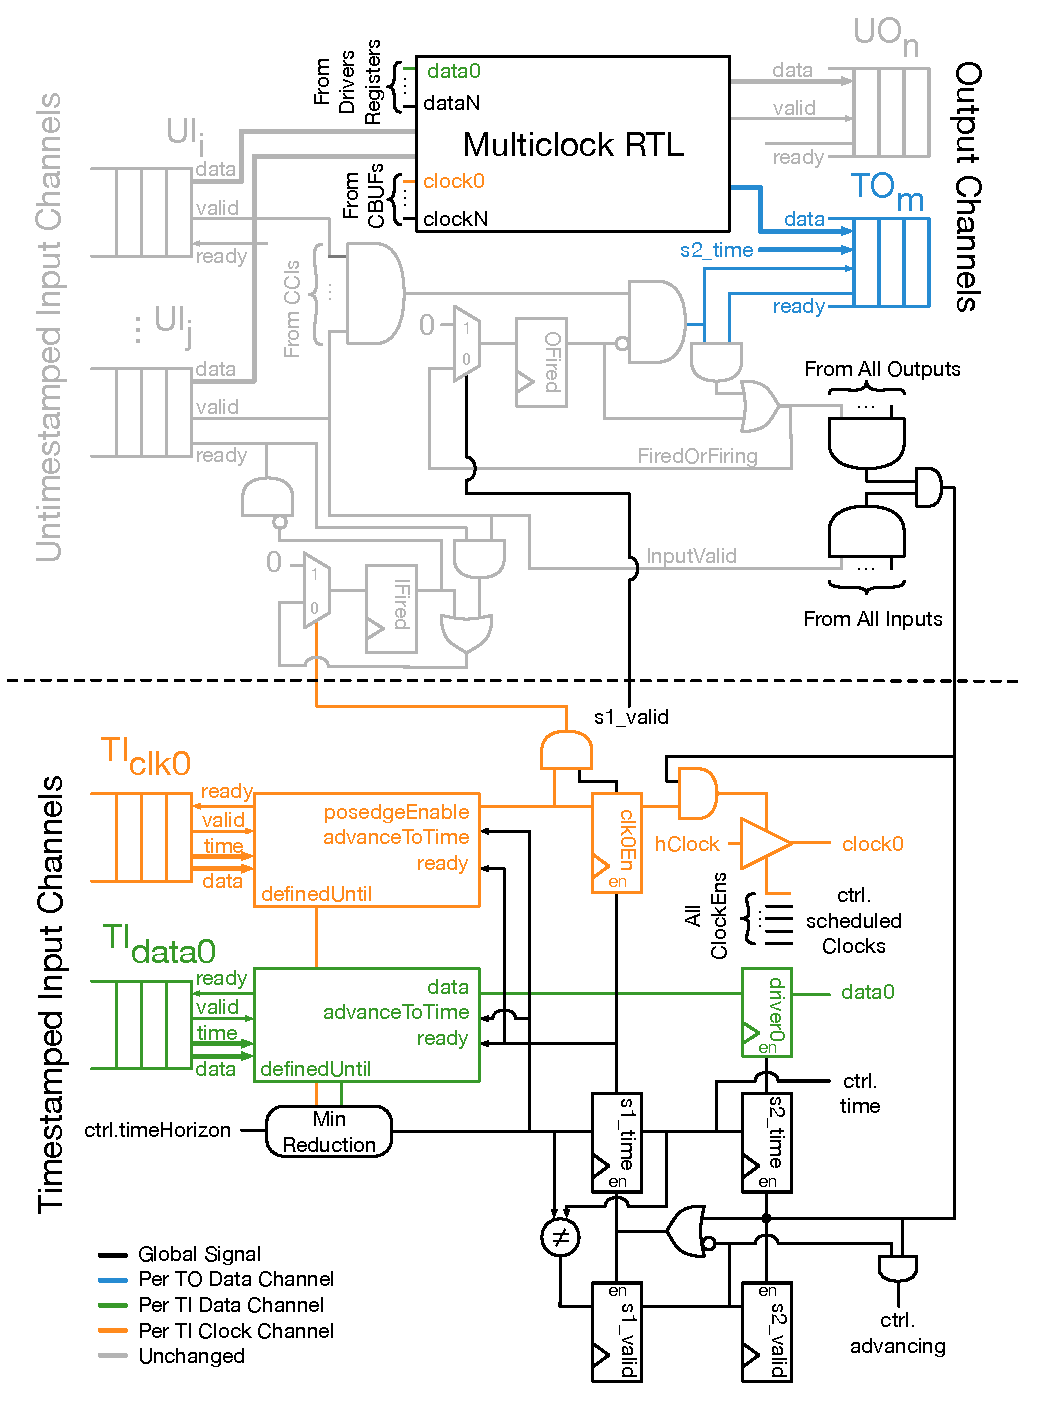
\includegraphics[width=0.99\textwidth]{figures/pdes-wrapper.pdf}
    % graffle2pdf -c pdes-wrapper midas-graphics/graffle/wrapper-transforms.graffle figures/pdes-wrapper.pdf
    \caption{The updated hub-unit wrapper. Circuitry in grey is unchanged from the multiclock
    wrapper we showed in Figure~\ref{fig:static-multiclock-wrapper}}.
    \label{fig:pdes-wrapper}
\end{figure}

We show the updated hub model in Figure~\ref{fig:pdes-wrapper}. The front-end
of the control pipeline~(bottom) consists of a series of schedulers that
unpack messages to provide the horizon over which an input is
defined~(\texttt{definedUntil}) and detect transitions.  If an input message
produces a transition it is not dequeued: the scheduler sets
\texttt{definedUntil} to that message's timestamp and waits. Conversly, null
messages and negative-edge transitions in clock-type channels are dequeued
upon arrival allowing that input's horizon to further advance. When no message is available,
\texttt{definedUtil} is set to the timestamp of the last message.

With the inputs unpacked, the fron-tend now a min-reduction across the horizons of all timestamped
inputs and an upper bound provided through the control
interface~(\texttt{ctrl.timeHorizon}).  This becomes the candidate time for the
next timestep and is broadcast back to each
scheduler~(\texttt{advanceToTime}).  If the pipeline can advance, all schedulers
with a transition or positive clock edge at the scheduled time dequeues their
input messages, and has their updated signal value latched.  The concatenation of all
enabled positive edges (\texttt{posedgeEnable}) corresponds to a clock token in
the sense defined in the previous chapter. Note that it is possible for there to exist no
transitions in a given timestep, it is scheduled anyway for reasons we will
discuss momentarily.

The "clock token" and data updates are scheduled and flow through the pipeline
as in the previous chapter (note, the first stage of the pipeline for data values is absorbed into the scheduler).
Untimestamped input~(UI) and output~(UO) channels handling
has not changed, their control FSMs are only reset when their clock has been
scheduled to fire. One critical implication of this is that asynchronous events
launched by data-type transitions in a particular domain do not launch new
tokens in untimestamped channel. This is consistent with our previous
assumption, from Section~\ref{sec:pdes-assumptions}, that untimestamped channels are driven by state elements that only
under go synchronous transtions with the channel's associated clock.

Timestamped outputs are managed differently. To avoid certain deadlock
conditions, TOs generate a new message on every timestep,
notably those in which no clock or data transitions have been scheduled. In
effect, these outputs have their FSMs reset on every timestep~(via \texttt{s1\_valid}), and source their
timestamp from the pipeline~(\texttt{s2\_time}).  Without further
optimization, this baseline hub unit gaurantees that output channels will
always be defined only as far as it oldest timestamped input.  Critically, this
means the hub unit has zero lookeahead. Thus to avoid deadlock,
any arc of timestamped units that begins and ends at the hub must provide non-zero lookeahead.

To provide finer-grained control and instrumention of the hub, we plumb out
specific signals to a memory-mapped simulation controller. This controller can
detect whether clocks are scheduled to fire~(\texttt{ctrl.clocksActive}), the
time of the associated timestep~(\texttt{ctrl.time}), and is responsible for
setting the aforementioned time upper bound~(\texttt{ctrl.timeHorizon}). This permits the controller
enable pausing the hub at specific times.

\subsection{Compiler And Annotation Modifications}\label{sec:pdes-compiler-modifications}

\begin{figure}
    \centering
    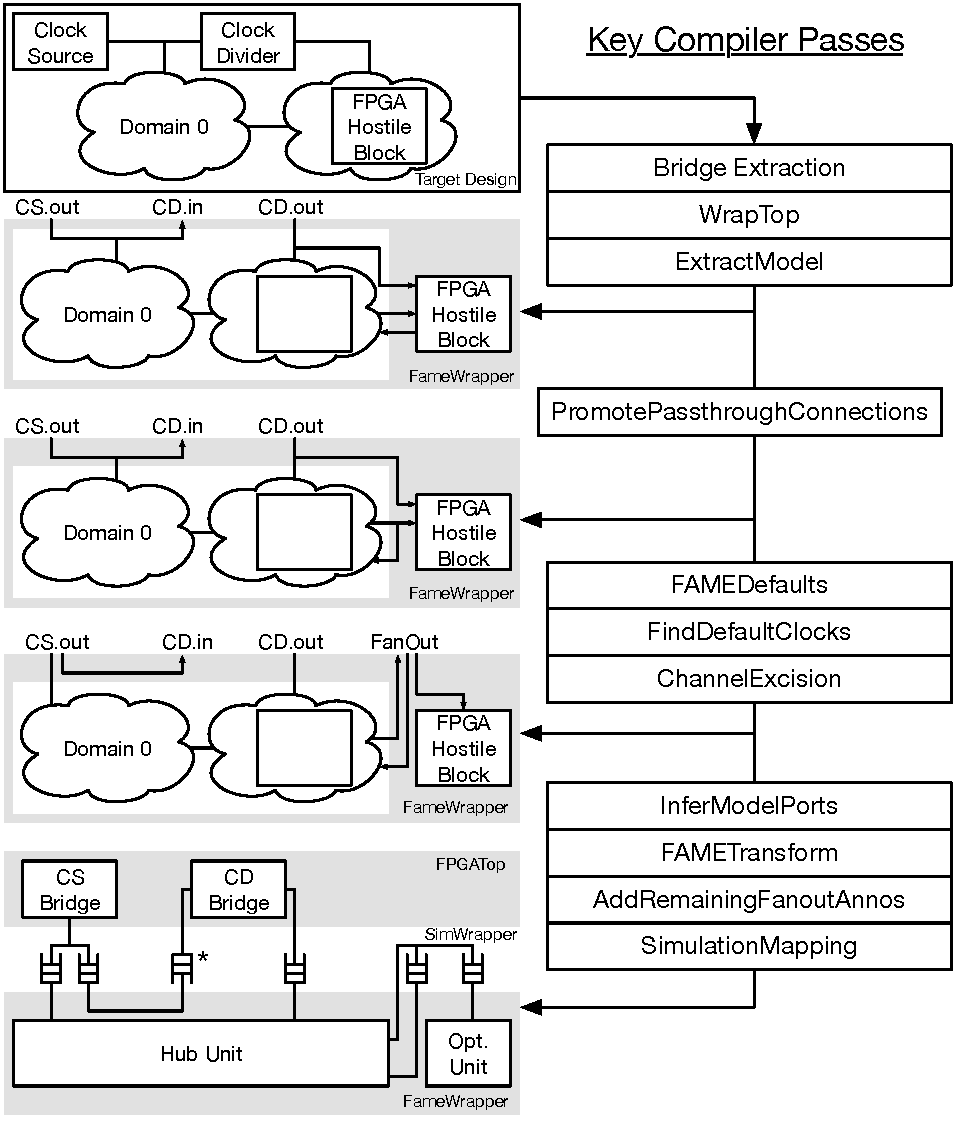
\includegraphics[width=0.99\textwidth]{figures/promote-passthroughs.pdf}
    % graffle2pdf -c main midas-graphics/graffle/promote-passthroughs.graffle figures/promote-passthroughs.pdf
    \caption{A visualization of the promote passthrough optimization.
    Modifications to the target are shown on the left at key points during
    compilation. We include a passthrough path in a optimizable block (right)
    to show how this transformation is broadly applicable to all inter-unit
    connectivity. Note, there is an extra channel generated (asterisk) in the
    bridge-to-bridge case currently, this can be optimized away in a future change.}
    \label{fig:promote-passthroughs}
\end{figure}

At a first blush, baseline support for timestamped channels is relatively
straightforward to implement. Since all timestamped channels are wire-type, the
timestamp of message can be treated as target-data in an otherwise coventional
token, and wiring between channels and bridges can be left unchanged. However,
to provide a workable baseline implementation, we need timestamped units to be
directly connected to one another, and not indirectly through the hub.  This
will permit timestamped units to advance ahead of the hub unit (which in its current form has zero lookahead).
Our earlier assumption that only timestamped units
can source clocks and signals that launch aynschronous events, lets us ensure that sources are only
ever directly connected to their sinks (~i.e., through a series of firrtl
\texttt{Connect} statements) and makes it easy to find and extract these these
paths into point-to-point channels between to units. We refer to this enhancement
as the \emph{passthrough connections optimization} and give a pictorial representation of the process in Figure~\ref{fig:promote-passthroughs}.

The core of this change revolves around the
\texttt{PromotePassthroughConnections} transform, which extracts wires of any FIRRTL type that
passthrough any top-level SSM. We run this pass in target transformation, after bridge and model extraction.
Note, if a signal drives no other sinks aside from output ports, we leave the
input connection instead of removing the connectivity altogether.  This
simplifies connectivity analyses that occur later in the compiler, and ensures
that all clocks still drive the hub (even if all of the state for a particular
domain has been extracted).

At this point top-level connectivity in the design now includes fanouts. To
handle this new class of connectitity we modified \texttt{ChannelExcision}. In
general, a fanout of $N$ produces one output interface, and N input interfaces
(sunk by the hub unit and optimized models) on the FAMEWrapper~(see the
right-most fanout in Figure~\ref{fig:promote-passthroughs}). The resulting
channel annotations share the same \texttt{source} targets, but their \texttt{sink} targets point at unique
inputs.

While a model-driven fanout can be deduced by looking at the source fields of
channel annotations, this does not apply to a bridge-driven fanout (since
bridge-driven channels leave their \texttt{sources} field empty).  Since
bridges are already removed (they are interfaces on the FAMEWrapper), a
bridge-sourced fanout of $n$ produces $n$ inputs and no output interfaces. The clock-source-driven interface (CS.out) in
Figure~\ref{fig:promote-passthroughs} is an example of this.
To reassociate these inputs with a single source, we organize bridge-driven
sources into fanout annotations~(\texttt{FAMEChannelFanoutAnnotation}). This
allows simulation mapping to drive the correct set of input interfaces from the
same bridge source. For consistency, we emit the same annotations for
unit-driven fanouts~(\texttt{AddRemainingFanoutAnnos}).

%differences between bridge vs model connectivity, added unneeded complexity by
%handling bridges liek models, and promoting their black-boxes into the
%FAMEWrapper instead of completely extracting them\footnote{This is a vestige of
%transtioning from MIDAS endpoints to Bridges}, which could happen later in the
%compiler. Here

Since this optimization now removes passthrough clock paths in models, a
model's target clock will be driven not from the hub, but instead from a
timestamped model (as seen in the FPGA hostile block in
Figure~\ref{fig:promote-passthroughs}). To this end we modified
\texttt{FindDefaultClocks}. The clock fields of intra-model channels must be
inferred by finding a clock sink port on the hub that shares the same source as
the clock sink on the model. This works because, as we previously suggested,
\texttt{PromotePassthroughConnections} ensures that all clocks remain
driven to the hub, even if all of the state associate with that domain has been
extracted from the hub.

The final necessary change for this optimization was to generalize the
FAMEtransform's re-wiring of the FAMEWrapper, which previously relied on the
assumption that all channels had sourced by a unit and sunk by a top-level
interface (or vice versa).

The optimization, while critical for the implementation of this dissertation
work, can improve FMR in the static-multiclock implementation when using using
bridges and / or multi-cycle optimizations that are directly connected to one
another.  Since, inter-model, or bridge-model, paths need not propagate through
the hub model first. In target in which a passthrough path would pass from hub,
to a model, and back to hub with no other combinational paths that span), FMR
improves from a best case of three to two. This improvement becomes more
pronounced for paths that run through a cascade of connected models. This
optimization has been upstreamed to mainline FireSim in version 1.12.

\subsection{Baseline Timestamped Units}\label{sec:pdes-baseline-units}

Writing timestamped units is the most difficult aspect of building out
these PDES simulators.  Many of the aforementioned difficulties associated with
writing multi-cycle models and bridges models apply, however timestamped units
must not only robust against not only changes in message arrival times (latency
insensitive), but they must be able to tolerate the presence of additional null
messages without changing their non-null output message streams. In
untimestamped units, the designer must manage cycle-scale decoupling (for
example, that the output has advanced some number of cycles ahead of the
input), whereas in timestamped models this decoupling is considerably
finer-grained. Additionally, whereas SSMs without combinational loops have well defined
outputs for a given input trace, this is not true of many of the circuits we
wish to model here. One specific example of this is that there can often be
race conditions that arise in due to simultaenous arrival of different inputs.
This can produce non-deterministic simulation behavior that is still is
compliant with Verilog's event ordering model. Since determinism is
critical for making FireSim simulations debuggable, the designer is forced to pick a
behavior.  Finally, timestamped units must find sufficient lookahead in their
reference RTL to avoid deadlock and provide good simulation performance.

We built our baseline TUs using a modular approach that would make it easy
to rewrite verilog implementations as timestamped units. Specifically, we
built a library of utilities to manage and unpack message streams, and
timestamped circuit primitives for registers, single-output combinational logic
functions, and fanouts. For each of these primitives we wrote deterministic Verilog
reference implementations, and built timestamping hardware to generate a
message stream from the reference hardware that could be compared against unit
output as part of a dynamic verification flow.

An important qualification is that these initial implementations we omit
asynchronous reset. While not insurmountable, async reset poses a key challenge to
our approach as it tends to remove lookahead opportunties affored by target
state. In leiu of this, we rely on FPGA programming or host-reset put TUs in
desired fixed starting state.  We discuss the complexity of modelling async
reset in these timestamped units in Future Work~(Section~\ref{sec:pdes-future-work}).

\subsubsection{Timestamped Tuples: Unpacked Messages}
Message streams are difficult to directly act upon, as in general, we are often interested
in data values between messages. One reasonable approach is to insert incoming messages into a
age-ordered event queue (as a software implementation would) and update TU state in message order.
In our timestamped units we went with a distributed approach, in which we wrote ad-hoc state machines to schedule over per-input
datastructures and avoids serialization on a single event queue
Given our baseline message encoding it is not possible to
detect transitions in a signal without comparing it an older value.  So these
hardware datastructures, which we refer to as \emph{timestamped tuples}, ease
this process by holding hold a pair of messages: the latest message (the head
of the channel's queue), and the previous message. When a unit wishes to
process events created by a non-null input message, it asserts \texttt{ready},
which moves the latest message into the secondary slot and the next message in
the queue becomes visible. At the point the former \texttt{previous} message is no longer visible,
and cannot affect output messages and internal state changes.

Unlike early conservative PDES work, in which lookahead in an LP statically
defined, our TUs can dynamically extract lookahead based on the values of
currently visible inputs. This is a domain-specific optimization akin to that
first described by D. Nicol~\cite{ImplicitLookahead} and B.
Lubachevsky~\cite{ImplicitLookahead2}. To describe lookahead properties of our
library primitives, it is useful to describe variables that derive simply
timestamped tuples. Suppose we have an input $I$, we define:

\begin{itemize}
    \item $T_{I}$ to be the time of the latest message. We refer to this as the \emph{horizon} of $I$.
    \item $P_{I}$ to be the time of the previous message.
    \item $I_H$ to be the data value of $I$ at its horizon.
    \item $I_P$ to be the data value of $I$ before its horizon, and defined at least as far as $P_I$.
    \item $I(t)$ to be the data value of $I$ at time $t$, where:
\end{itemize}
\[ I(t) = \begin{cases}
    I_H & \quad \text{if } t = T_{I} \\
    I_P & \quad \text{if }  T_{I} > t \geq P_{I} \\
    undefined & \quad \text{otherwise} \\
\end{cases}
\]

\subsubsection{Edge-Triggered D Flip Flops}
D flip-flops, both positive and negative-edge triggered, are critical elements for
building integer clock dividers and clock muxes. Our basic timestamped model has three compile-time parameters:

\begin{itemize}
 \item \textbf{Data type:} the chisel-type the register can hold.
 \item \textbf{Initialization value:} The value the register assumes at time 0.
 \item \textbf{Edge sensitivity:} this can be set to either postive or negative edge sensitive.
\end{itemize}

Structurally, it has a clock type input, and a data type input (D) and output
(Q) of the data type above.  This primitive models no clock-to-Q delay, and so
an output transition on Q occurs simultaenously with a latching edge.  In other
words, the input clock message and output Q message share the same timestamp.
Additionally, this register observes the value of D one timescale unit before
the positive edge. Thus if a clock and data transition occur simultaenously,
the clock always observes the old value of D.  This is often a data-race in a
Verilog expression of a Flip-Flop as the assignment to D and the evaluation of
RHS of a non-blocking assingment to Q can be executed in either order. Our
implementation ensures the non-blocking RHS evaluation occurs first.
Critically, this gauarantees that the flip flop has non-zero lookahead when the
clock input leads the D input. We give the rules governing the timestamp of an
output message based on the available inputs, and thus the available lookahead,
below:.

\begin{algorithmic}
    \If {$T_{clock} \geq T_{D}$}
        \If {$\text{Clock} = \text{latching edge} \textbf{ and } (T_{clock} - T_{D}) > 1$}
            \State $t_{L} = (T_{clock} - 1) - T_{D}$
        \Else
            \State $t_{L} = T_{clock} - T_{D}$
        \EndIf
    \Else
        \If {$D_H = Q_H$}
            \State $t_{L} = T_{D} - T_{clock}$
        \Else
            \State $t_{L} = 0$
        \EndIf
    \EndIf
\end{algorithmic}

Using the information encoded in the message streams alone this register's
output cannot always advance ahead of both Clock and D. However, this model
does have non-zero lookahead relative to D, which will suffice to avoid
deadlock in many important classes of designs we will discuss in
Section~\ref{sec:pdes-common-circuit-perf}.  We note, the most natural way to
introduce clock-relative lookahead, if required, is to model a clock-to-Q
delay. Similarly, D-relative lookahead could be improved by having the model
observe the D earlier relative to the clock edge, as the path will need to meet
a reasonable setup time constraint to avoid metastability.

\subsubsection{Generic Combinational Functions}
Our baseline schedules over a set of timestamped tuples, and generates a single
output message at the timestamp of the oldest input message. This
implementation is conveninent in that the user can generate arbitrary
combinational logic over all input tuples, however this comes at the cost of
having zero lookeahead as its output is defined only as far as its oldest input.

Without providing additional hints about input transitions, there are two
mechanisms for finding more lookahead.  The first is modeling propoagation
delays through gates. Here, $$t_L = \min_{\forall I} (T_{I} + minPD_{I})$$
where $minPD_{I}$ is the minimum propogation delay of the circuit from input $I$ to
the output.  The second means is to leverage logic redundancy. If the oldest
input to a combinational funtion cannot not affect the output (i.e., it can be
treated as a dont care) the output can advance ahead of that input.

\subsubsection{Fan Outs}
To broadcast a tuple from one source to many sinks, we wrote a fanout
primitive. Under the hood, this repacks the tuple into a message that is then
broadcast to a set of queues, much in the same way a fanout channel is
implemented in in the simulation wrapper. These queues are of finite depth, and
must be sized conservatively by the designer to avoid deadlock.

\subsubsection{Fixed-Period Clock Sources}

This primitive is reponsible for generating an infinite trace of clock messages. It has the following
compile-time parameters:
\begin{itemize}
 \item \textbf{Period:} The clock period in picoseconds.
 \item \textbf{Initialization value:} The value the clock assues at time zero.
 \item \textbf{Duty cycle:} the percent of the time the clock is high.
\end{itemize}

Having only a single clock output and no inputs, it effectively has infinite
lookahead and can run arbitarily far ahead of other timestamped units in the
graph.  Of the primitives listed above, this is the only one with a wrapper
\texttt{BridgeModule}, and so can be used in target RTL.

\subsection{Library Timestamped Units}
Using these library primitives we built simple TUs by translating verilog
primitives to timestamped equivalents. We give an example of this using a
phase-aligned by-two clock divider: its reference verilog is shown in
Listing~\ref{lst:verilog-clock-divider} and its timestamped translation is
shown Listing~\ref{lst:tu-clock-divider}. Using this scheme, we also baseline
TUs for by-three (Figure~\ref{fig:by3-clock-div}) clock dividers, a glitchless
two-to-one clock mux~(Figure~\ref{fig:clock-mux-glitchless} and an and-based,
ICG~(Figure~\ref{fig:clock-gate}).  Note that the output clock in each of these
circuits is not combinationally dependent on a control input: this ensures a
cycle that spans the hub and a TU modelling one of these circuits has non-zero
lookahead.

\begin{lstlisting}[language=Verilog, style=verilogStyle, float,
label={lst:verilog-clock-divider}, caption=A reference phase-aligned clock-divider from Rocket Chip used in RTL simulation.]
module ClockDivider2 (output reg clk_out, input clk_in);

   initial clk_out = 1'b0;
   always @(posedge clk_in) begin
      clk_out = ~clk_out; // Must use =, NOT <=
   end

endmodule // ClockDivider2
\end{lstlisting}

\begin{lstlisting}[language=Scala, style=scalaStyle, float, label={lst:tu-clock-divider}, caption=The equivalent timestamped unit for the clock divider shown in Listing~\ref{lst:verilog-clock-divider} implemented using library primitives.]
class ClockDivider2 extends MultiIOModule {
  val clk_in   = IO(Flipped(new TimestampedTuple(Bool())))
  val clk_out  = IO(new TimestampedTuple(Bool()))
  val reg = Module(new TimestampedRegister(Bool(), Posedge, init = Some(false.B)))
  reg.simClock <> clk_in
  val Seq(feedback, out) = FanOut(reg.q, "feedback", "out")
  clk_out <> out
  reg.d <> (new CombLogic(Bool(), feedback){
    out.latest.bits.data := ~valueOf(feedback)
  }).out
\end{lstlisting}

\begin{figure}
    \centering
    \begin{subfigure}[t]{0.35\textwidth}
        \captionsetup{margin=0.25cm}
        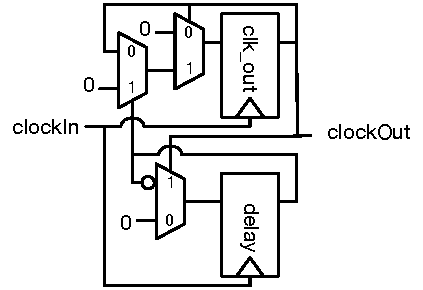
\includegraphics[width=\columnwidth]{figures/clock-div3.pdf}
        \caption{By-3 clock divider.}
        %graffle2pdf -c clock-divider-3 midas-graphics/graffle/clock-muxes.graffle figures/clock-div3.pdf
        \label{fig:by3-clock-div}
    \end{subfigure}
    \hspace{-1cm}
    \begin{subfigure}[t]{0.40\textwidth}
        \captionsetup{margin=0.25cm}
        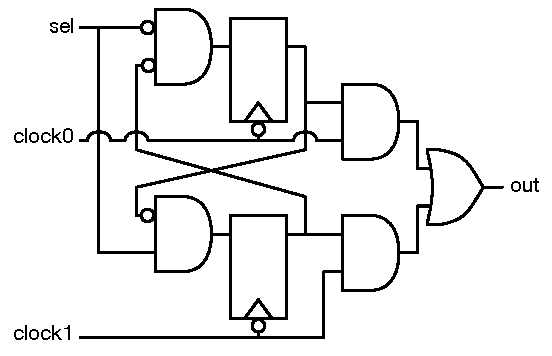
\includegraphics[width=\columnwidth]{figures/clock-mux-glitchless.pdf}
        \caption{Glitchless clock mux.}
        %graffle2pdf -c glitchless midas-graphics/graffle/clock-muxes.graffle figures/clock-mux-glitchless.pdf
        \label{fig:clock-mux-glitchless}
    \end{subfigure}
    \hspace{-1cm}
    \begin{subfigure}[t]{0.30\textwidth}
        \captionsetup{margin=0.25cm}
        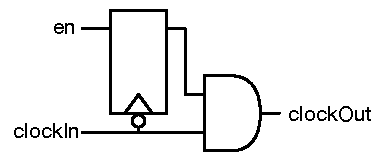
\includegraphics[width=\columnwidth]{figures/clock-gate.pdf}
        \caption{Clock-gating cell.}
        %graffle2pdf -c clock-gate midas-graphics/graffle/clock-muxes.graffle figures/clock-gate.pdf
        \label{fig:clock-gate}
    \end{subfigure}
    \centering
    \caption{Reference circuit diagrams for the baseline TUs. Verilog for the
    by-2 divider is provided in Listing~\ref{lst:verilog-clock-divider}, so we
    omit it here.}
    \label{fig:baseline-reference-circuits}
\end{figure}

\subsection{Verification}

We relied on dynamic verification to check our implementations. We
wrote a SystemVerilog "timestamper" which transates a signal into a decoupled
message stream, by leverage Verilog's \texttt{\$time} system function to
produce a timestamp. We then wrote chisel testbenches to show to two message
streams were correct in the manner described in
Section~\ref{sec:lp-correctness}.
%We wrote fuzzers to inject both host-delays and additional null messages into message streams,

As we have mentioned, many of the aforementioned circuits have expected
non-determinsitic behavior when written in a conventional Verilog style. For
example, if the input to a D flip-flop transitions concurrently with a latching
edge transition, the RHS of the non-blocking assignment to the register and the updated
assignment to the wire can be legally executed in either order. This makes it difficult to write
deterministic, dynamic tests of these units. Thus, we wrote race-free
reference implementations which guarantee a particular ordering by judiciously adding sub-\texttt{time\_unit}
delays~(i.e., akin to delta cycles in VHDL parlance). This approach does not scale well to
compositions of these sub-circuits, but suffices to verify small circuits are
determinisitically represented by its timestamped unit.

\section{Performance in Common Clock Organizations}\label{sec:pdes-common-circuit-perf}

\begin{figure}
    \centering
    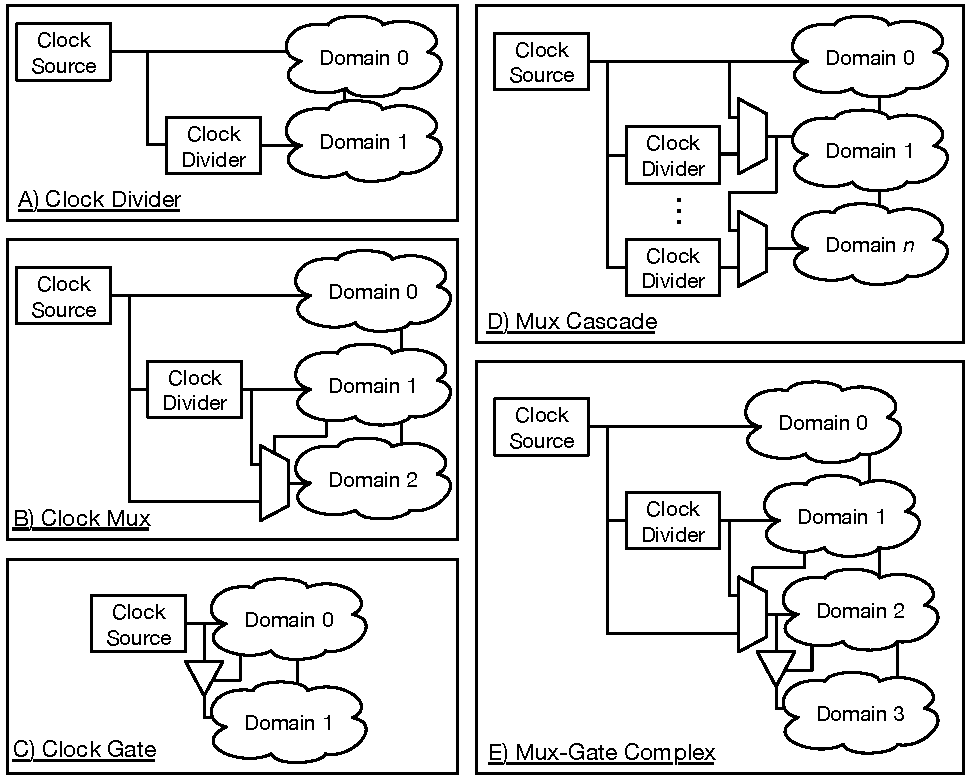
\includegraphics[width=0.99\textwidth]{figures/clock-organizations.pdf}
    % graffle2pdf -c combo midas-graphics/graffle/clock-organizations.graffle figures/clock-organizations.pdf
    \caption{}
    \label{fig:clock-organizations}
\end{figure}

What should be clear from the previous sections is that these baseline TUs are
conservative. Since they make no assumptions about the behavior of their
inputs, they cannot find lookahead in all of their input corners, specifically
in cases where a clock-type input is oldest input to the unit. Fortunately, in
many useful classes of clock organizations (depicted in
Figure~\ref{fig:clock-organizations}), there are no cycles that do not span the
hub unit. Since all of our units have non-zero relative lookahead relative to
their hub-driven control input, all of these circuits narrowly avoid deadlock.
Of course, this does not imply they simulate with a low FMR: here we measure
the performance of our prototype on the circuit organizations of
Figure~\ref{fig:clock-organizations}, and shed light on the origin of
performance losses where they exist. We summarize their FMRs in
Table~\ref{tbl:pdes-baseline-fmrs}.

\begin{table}[t]
\centering
    \begin{tabular}{c c c c c}
    \hline
          \textbf{Divider} & \textbf{Mux} & \textbf{Gate} & \textbf{3-Mux Cascade} & \textbf{Mux-Gate} \\
          3.0 & 11.0 & 6.0 & (12.5, 13.0) & 15.5 \\
    \hline
    \end{tabular}
    \caption{Measured FMR of the clock organizations shown in Figure~\ref{fig:clock-organizations} using the baseline TUs.}
    \label{tbl:pdes-baseline-fmrs}
\end{table}

\subsection{Feedforward Divider Networks}

A feedforward network of clock-sources and clock dividers
(Figure~\ref{fig:clock-organizations}, circuit A) is the simplest case, and
suffices to model the systems we described in the previous chapter. Performance
in these targets is bandwidth bound on the ability of the downstream dividers
to process input messages from the high-frequency reference clock. The baseline
by-two clock divider, reported in Table~\ref{tbl:pdes-baseline-fmrs} takes three cycles on average to process two input
messages (one reference clock cycle). This arises because the flip flop model, unware
that it is driving itself in a feedback loop, waits for it's D input to be defined one-time unit
before the next positive clock edge, introducing a single internal null
message. Thus, when the fastest clock is driving other logic in the target, the
best case FMR of these targets is three.

It is important to note that if we remove the fast clock domain (domain zero in
Figure~\ref{fig:clock-organizations}), from the user's perspective the FMR
doubles to six~(when using by-two clock divider). Unfortunately, cases in which
the high-frequency clock is not widely deployed in the target-design is a
common case. For example, in order to generate the 1.5, 1.0, and 0.75 GHz
clocks for the three-domain target SoC we described in
Section~\ref{sec:spec-perf}, we would be forced to generate a 3.0 GHz
reference, and then use by-two, by-three, and by-four (two by-twos) to generate
the target clocks. The cost of directly simulating the fast clock increases as
the ratio between the reference and the fastest derived clock grows. We describe

\subsection{Simple Hub Cycles}
Clock gates and clock muxes (Figure~\ref{fig:clock-organizations}, circuits B and C) create a
two-unit cycle in the simulator graph that span a hub-driven control signal and a
TU-driven clock. Performance in these configurations is latency-bound on
message transmission through this cycle and is further deteroriated by
null-message cycles that introduce additional transits through on each derived
clock cycle.

This is most clearly illustrated with the clock gate configuration, which has a
measured FMR of six. Both the reference clock and derived (gated) clock have
the same frequency: so the FMR of derived clock is not further bandwidth bound
beyond two. Any additional slowdown is the result of the clock-gate waiting on
message propagation from the hub. We show message propogation through the
simulator in Figure~\ref{fig:clocks-gate-control-loop}. Here the reference clock has a period of
four, and a there is a positive edge at $t = 0$. Since the hub must wait for
input message from both the source and the ICG TU, and since the ICG always
lags the source, we neglect the source in this diagram.

There are two effects at play here. After the ICG has enqueued a positive edge
message for its output clock at host cycle zero,  it takes four host cycles for
a enable message sharing that time ($t=0$) to arrive at the input. A transition
in enable would be visible in this message if it occurs. Unaware of this, the
register model in the ICG waits for an input defined one time\_unit before
clock's negative edge ($t >= 1$). This requires a null-message propagation (the
second message) to propagate through the loop. Once it arrives at host cycle 5,
the negative edge is processed and new enable is latched. In host cycle 6, the
second positive edge is finally enqueued. This cycle recur thus giving an FMR
of six.

\begin{figure}
    \centering
    \captionsetup{margin=0.25cm}
    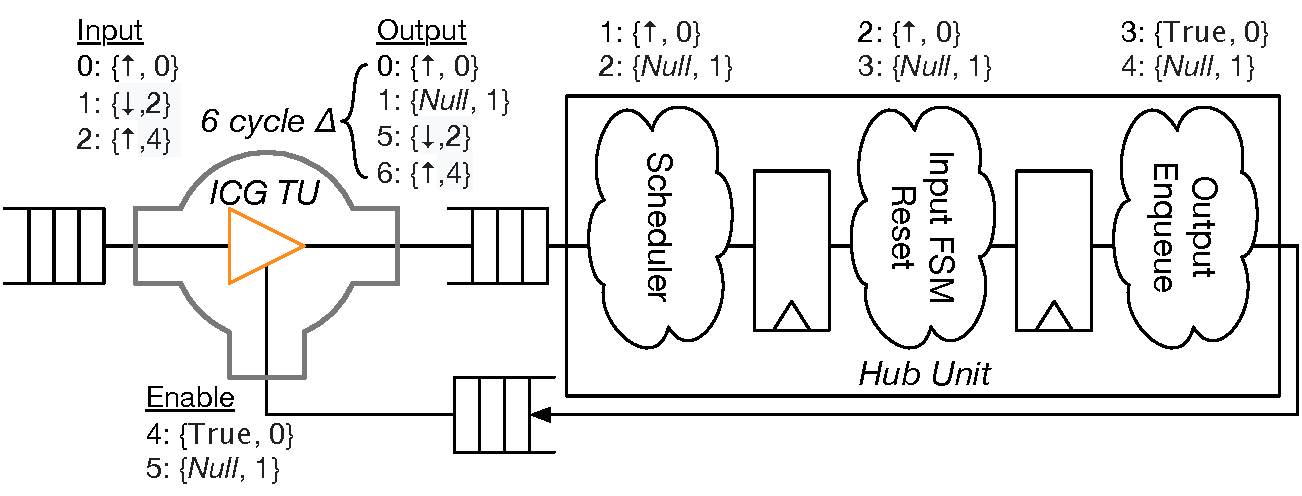
\includegraphics[width=\columnwidth]{figures/clock-gate-control-loop.pdf}
    \caption{}
    %graffle2pdf -c baseline midas-graphics/graffle/clock-gate-control-loop.graffle figures/clock-gate-control-loop.pdf
    \label{fig:clock-gate-control-loop}
\end{figure}

The clock mux configuration has significantly worse FMR~(11.0) because null-token propagation loops
are not always overlapped with the propagation of edge (as in the previous
example). In otherwords, a null-message received on the select input by the mux launches a second
null-message that must propagate through the simulator, instead of allowing the
unit to enqueue a new output edge.

\subsection{Multi-Unit Cycles}

Clock multiplexor cascades (Figure~\ref{fig:clock-organizations} D) and
multiplexor-gate complexes (Figure~\ref{fig:clock-organizations}) are also
common occurances in SoCs. Here cycles exist between a hub-driven control
signal, and multiple cascaded TUs, which terminates at a clock input on the
hub. One might expect that these topologies would have greater FMRs, since the
transmission time across the loop is longer, without extracting substiantially
more lookahead per TU crossed.

This is not always case with mux cascades when selecting between clocks of the
same frequency: it depends on which domain drives the select signal. When the select is driven by the same domain the mux drives,
these circuits run with an FMR of 11.0 independent of the depth of the cascade ($N$).
When select is driven by the previous clock domain, FMR increases to
13.0.  When each stage is fed by a different frequency, for instance with clock
divider with a division of $i+1$, where $i$ is the index of the current domain,
the story becomes more complicated. Here encreasing the cascade depth,
marginally increases FMR (12.5, 13.2, 13.2, from $N=3$ to $N=6$), due to the
introduction of new null-messages by the dividers themselves. Removing these
messages would return FMR to 11.0.

Topologically, the mux-gate complex is analagous to the
previous-domain-drives-select mux-cascade case mentioned previously, as the
clock enable cannot solely be driven state by the domain it is gating. Here we
measured an increase in FMR from 11 to 15.5 over the single mux case, because
the launch of an enable message serialized directly behind the selection of a
clock. Indeed, the primarly driver of increased FMR is not the length of a
cycle, which can be problematic, but rather tight coupling clock generation and
the control logic.

\subsection{Compositions Of Circuits}

We speculate that, in general, the circuits we present in
Figure~\ref{fig:clock-organizations} can compose with zero or modest increase
FMR if they derive from the same clock source, or from a second clock source
that is a phase-aligned integer division of the source. This is because their
message propoagation happens in parallel, and few, if any, new simulator
timesteps are introduced. More complex compositions that derive from a clock
driven by a clock mux or clock gate require more detailed analysis, as
depending on which domains drive control signals. This effect is visible
already manifest in both the mux-gate complex and mux cascade circuits.

\section{Lookahead Optimized Units}\label{sec:pdes-opt-units}
While there are systemic approaches for improving simulation performance in our
baseline implementation, the lowest hanging fruit revolve around optimizations
that can extract more lookahead non-hub TUs. Without introducing logic or
propagation delay, this must rely upon exploiting the presence of state in the
reference circuits which provide a multi-period interval of
opacity~\cite{ImplicitLookahead2} wherein changes in the hub-driven control
signal are not observable in the output message stream. While it may be
possible to automatcally  generate a lookahead-optimized model in the future,
here we throw out the library primitives in favor of a fully handwritten ones.
The cost of this approach is that writing correct TUs becomes more challenging,
as these units cannot be simply transcribed from verilog.

\begin{table}[t]
\centering
    \begin{tabular}{c c c c c c}
    \hline
%           & \textbf{Divider} & \textbf{Mux} & \textbf{Gate} & \textbf{3-Mux Cascade} & \textbf{Mux-Gate} \\
%          Baseline        & 3.0 & 11.0 & 6.0 & (12.5, 13) & 15.5 \\
%          Opt. Dividers   & \textbf{2} & 11.0          & ---        & (\textbf{13}, 13)             & 15.5 \\
%          Opt. ICGs       & ---        & ---           & \textbf{4} &  ---                          & \textbf{14.0} \\
%          Sync Mux $k=1$  & ---        & \textbf{2.63} & ---        & (\textbf{3.0}, \textbf{4.75}) & \textbf{5.28} \\
%          Sync Mux $k>=2$ & ---        & \textbf{2}    & ----       & (3.0, 4.75)                   & \textbf{4.97} \\
           & \textbf{Divider} & \textbf{Mux} & \textbf{Gate} & \textbf{3-Mux Cascade} & \textbf{Mux-Gate} \\
          Baseline        & 3.0 & 11.0  & 6.0 & (12.5, 13.0) & 15.5 \\
          Opt. Dividers   & \textbf{2.0} & 11.0          & ---        & (\textbf{13}, 13)             & 15.5 \\
          Opt. ICGs       & ---          & ---           & \textbf{4.0} &  ---                          & \textbf{14.0} \\
          Sync Mux $k=1$  & ---          & \textbf{2.6}  & ---        & (\textbf{3.0}, \textbf{4.8}) & \textbf{5.3} \\
          Sync Mux $k>=2$ & ---          & \textbf{2.0}  & ---       & (3.0, 4.8)                   & \textbf{5.0} \\
    \hline
          All & 2.0 & 2.0 & 4.0 & (\textbf{2.0} \textbf{2.8}) & \textbf{2.7} \\
    \end{tabular}
    \caption{Measured FMR of the clock organizations shown in Figure~\ref{fig:clock-organizations} using the baseline TUs.}
    \label{tbl:pdes-baseline-fmrs}
\end{table}

\subsubsection{Integer Clock Dividers}
If we continue to neglect asynchronous reset, it is trivial to write a
clock-divider model that can consume an input message per cycle. Our optimized
TU always dequeues messages that do not encode positive clock-edges. On
positive clock edges, the TU increments a counter, and if the counter has
reached a threshold for a positive or negative output edge, it supplies the
appropriate output message.  Otherwise, it greedily enqueues output
null-messages stamped to the arrival time of the last input clock edge.
Assuming an input message stream that has no null-messages, the only
circumstance under which this unit cannot process an input edge per host-cycle
is if there is backpressure on non-null output messages.

\subsubsection{Integrated Clock-Gating Cells}
A typical latch-based clock gate is difficult to optimize because the the latch
is transparent in the half-period directly before an input positive edge. As a
result, late arriving enable signals produce observable changes in the output.
Indeed, the latch exists to soley to prevent glitches in the output clock, so
from a lookahead pespective it is more illustrative to think of this circuit as
a combinational and of its inputs.  To avoid this, in our
primitive model, we used a negative-edge-triggered D flip flop instead of a
latch, which provides a half-period of lookahead.

Without introducing delays on propagation or latch behavior, the only recourse
the unit designer has is to exploit knowledge about the behavior of the input
message streams. Here the main observation is that the clock enable function
tends to be synchronous to the input clock.  If this is the case, and the
enable signal is being driven by the hub, there should eventually be an input
message with the same timestamp as the input positive edge that launched it.
Where as the general implementation must wait until one time-unit before the
next positive edge, in this case, we can lookahead one input cycle, removing
the need to wait for null-messages to arrive that ensure there are no further
changes in the enable before the arrival of a negative clock edge.

\subsubsection{Clock Multiplexors}
%At their core, simple clock multiplexors~(Figure~\ref{fig:clock-mux-naive}) suffer from the same challenges as clock
%gates, with edges in the output clock being defined by a combinational function
%on the input clocks and select.
Our baseline clock multiplexor based on circuit in
Figure~\ref{fig:clock-mux-glitchless}, extracts the smallest degree of
lookahead available to avoid deadlock. While a handwritten model could do
better by exploiting knowledge of the feedback loop between the two
clock-enable registers. To do better still, we can model a multiplexor that
remains opaque to changes in the select signal for a longer period of time.
This is true of typical glitchless clock muxes designed to switch
unrelated clocks (Figure~\ref{fig:clock-mux-sync}). Here the clock select must be first sychronized
to each clock domain, before it produces an observable change in the output
clock.

\begin{figure}
    \centering
    \captionsetup{margin=0.25cm}
    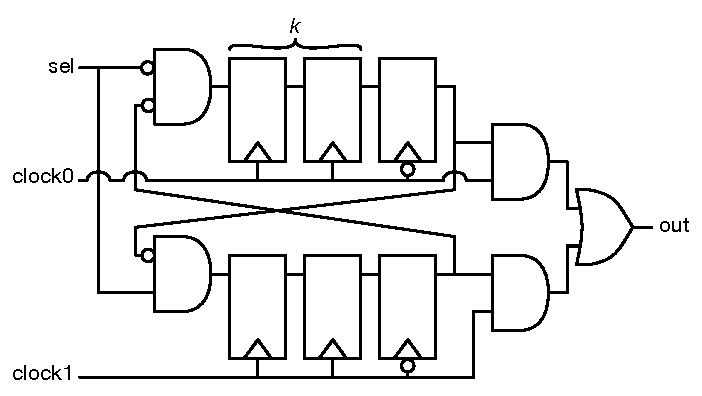
\includegraphics[width=0.6\columnwidth]{figures/clock-mux-sync.pdf}
    \caption{A synchronized, glitchless two-to-one clock multiplexor that can safely switch between two unrelated clocks.
    $k$ is the length of the synchronizer chain.}
    %graffle2pdf -c sync midas-graphics/graffle/clock-muxes.graffle figures/clock-mux-sync.pdf
    \label{fig:clock-mux-sync}
\end{figure}

We built a custom unit to model this variety of clock muxes that is
configurable in the number of clocks it switches between ($n$), and the depth
of the synchronizer chain~($k$). Our unit consists of $n$ clock handlers, each
of which dequeue input messages up to $k$ positive edges in advance of the
select.  In steady state, a clock edge $k$ periods in the future of the current
clock select value can be driven to the output.  On a transition no further
clock edges are presented. Instead, after a negative edge for currently
selected clock has been sent, a null message corresponding to a dead period of
$k$ periods in the new clock domain is emitted. At this point, positive edges
for the newly selected domain are made visible as they arrive at the clock
handler. The choice of $k$ is the key determiner of the available lookahead in
this variety of multiplexor. We revisited the circuit topologies using muxes
from Section and re-evaulated them using this new TU.

\section{FPGA QoR And Scalability}

Much of the feasilbility of our approach relied on the assumption that managing
large timestamps for relatively few and small TUs, would incur a small resource
cost relative to the rest of the simulator. Here we quantify these costs by
measuring TU and hubunit utilization, and reporting their $f_{max}$ when
synthesized in isolation.

% Vivado version

\subsection{TU Resource Utilization}
One would expect that building TUs that process multiple streams of messages
with large timestamps would bring about a large resource cost, despite the
underlying simplicitly of the target circuits they model. We measure LUT and
register utilizations for all of the TUs we've built, and report them in \TODO{Figure}.

\begin{table}[t]
\centering
    \begin{tabular}{c c c c c}
        TU & Logic LUTs & Registers & Memory LUTs & $f_{max}$ \\
    \hline
        Clock Source & 38 & 63 & 0& 200 \\
        \hline
        ICG Baseline  & 1134 & 283 & 84& 128 \\
        ICG Optimized & 260 & 131 & 0& 200 \\
        \hline
        Clock Mux & 3372 & 1084 & 420& 164 \\
        Clock Mux (Sync, $k=3$) & 911 & 82 & 80& 200 \\
        \hline
        Divider (By 2) & 986 & 282 & 84& 200 \\
        Divider (By 3) & 2527 & 793 & 294& 153 \\
        Divider Optimized & 40 & 67 & 0& 200 \\
    \hline
    \end{tabular}
    \caption{}
    \label{tbl:pdes-tu-utilization}
\end{table}

As a fraction of the resources available on the VU9P, TUs utilization is
insignificant, even when using a wider 64-bit timestamp.  For large networks
this cost may grow: using a more optimized message  encoding and TU
implementations that avoid acting directly on absolute times, would likely
suffice to remove most of this cost. These units indepedently close timing at
frequencies far higher than other parts of the systems we typically simulate,
and are unlikely to ever aversly affect $f_{fpga}$. The same cannot be said of
the hub unit, which we explore next.

\subsection{Hub Unit QoR And $f_{max}$ Scaling}
Another scaling challenge of our approach are costs associated with the
front-end of the hub unit's pipeline, which features a large min-reduction
across timestamps. We measured the per-timestamped input scaling trends of the
hub by synthesizing a scan chain, where each register is asynchronously reset
by an independent source. This adds a new timestamped input per register in the
chain without using more BUFGCEs beyond the first. Here we build complete simulator bitstreams using FireSim's standard
build flow with the ``timing'' strategy and Vivado version 2018.3.

\begin{figure}
    \centering
    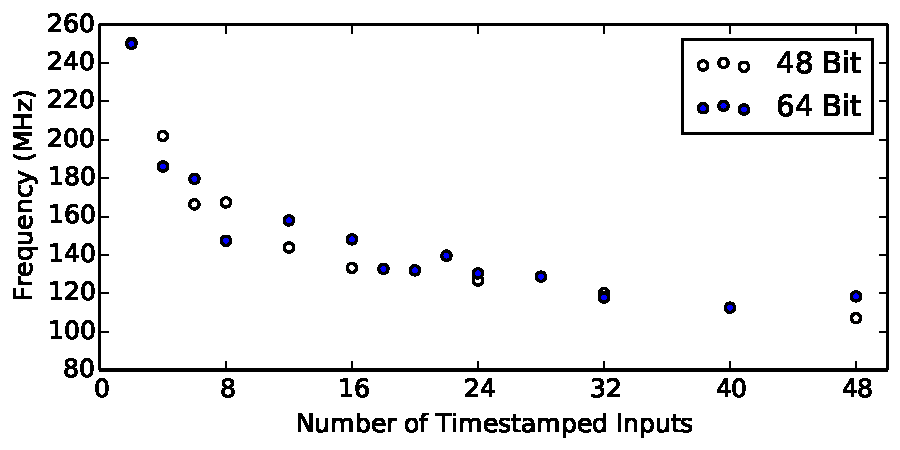
\includegraphics[width=0.6\textwidth]{figures/pdes--hub-fmax-scaling.pdf}
    \caption{}
    \label{fig:pdes-hub-fmax-scaling}
\end{figure}

In Figure~\ref{fig:pdes-hub-fmax-scaling}, we plot $f_fpga$ of the simulator as
a function of the number of timestamped inputs used under both 48 and 64 bit
timestamps. To produces these numbers, we coarsely overconstrained the
simulator clocks frequency (by up to 10 MHz in some cases). Given this
heavy-handed overconstraint and the inherently stochastic nature of FPGA place
and route, fluctuations in $f_{fpga}$ are expected. The overall trend is clear
however.  In both cases, Vivado can successfully close timing over 100 MHz up
to when using up to 49 timestamped inputs. This is well beyond the $f_fpga$ we
achieve when simulating large systems typically. Nonetheless, this may still be
a problem when synthesized alongside a more realistic target, where congestion
becomes more problematic. Practically speaking, global clock resource
limitations will prevent the hub's frontend from becoming the simulators
critical path. If we consider $N=12$, the point at which Vivado struggles to
place and route more global clocks, the simulators $f_{fpga}$ was 144 MHz and
158 MHz for 48b and 64b timestamped respectively. By comparison, recall that
with multi-cycle setup constraints the Rocket and Boom targets of the previous
chapter closed timing at 150 MHz and 90 MHz respectively~(and require fewer
global clocks).

\begin{figure}
    \centering
    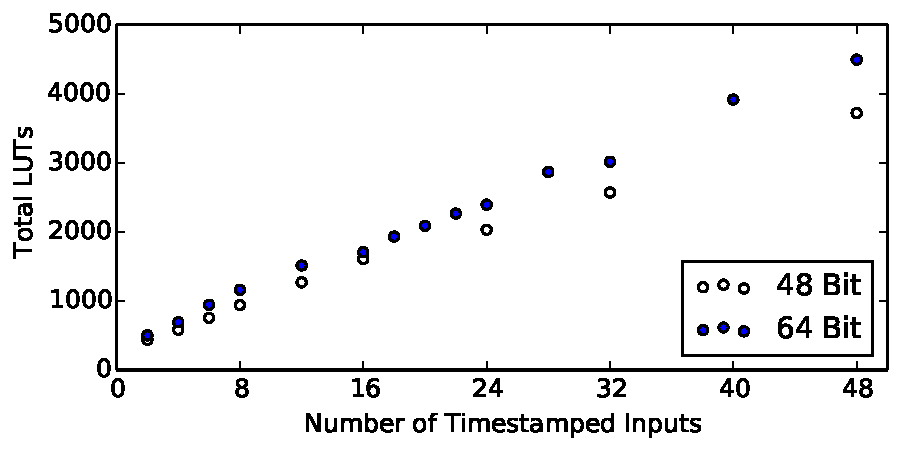
\includegraphics[width=0.6\textwidth]{figures/pdes-hub-lut-scaling.pdf}
    \caption{}
    \label{fig:pdes-hub-lut-scaling}
\end{figure}

Another potential concern is the LUT utilization of the frontend of the hub.
In Figure~\ref{fig:pdes-hub-lut-scaling}, we report LUT utilization of all
modules under the simulation wrapper versus the length of the scanchain. This
includes the hub, and channel implementations, but excludes all bridges and
FPGA-shell collateral like DRAM controllers. While some LUTRAMs are used to
implemented parts of the channels and hub, their use is light relative to logic
LUT utilization, so we omit them here. LUT utilization scales nearly linearly
with increasing input count with approximately 86 and 74 additional LUTs required per
timestamped input for 64b and 48b designs respectively. While not
insignificant, the 4494 LUTs used in the 48 input, 64b variant accounts for
just 0.38\% of the total available LUTs in the VU9P FPGA.

\section{Example Case Study}

The support we've described in this chapter unlocks fast, determinisitic
simulation of a large space of interesting systems. In this section, we show how this
could be used to study novel thermal management and DVFS policies, by
simulating a Chipyard SoC that uses frequency throttling to stay within a
desired thermal envelope. Our system is unique among academic works in it's generality and how 
relatively non-invasive it is: in principle no-simulation specific devices need
to be exposed to target software, and target drivers need not be modified for
FireSim since they continue to write to the same memory-mapped registers that
would be present in the actual chip. Of course, performance-accurate simulation is only
one half of this puzzle---a detailed power model is also required to complete
the loop. Prior work based on FireSim, notably Simmani~\cite{Simmani}, would be
a good fit if and when it is upstreamed into FireSim.  In leiu of a more
accurate power model, we've used a simple replacement which is sufficient to
demonstrate the work described in this chapter.

\subsection{Target SoC}
Here we simulate a single-core rocket-based SoC, shown in
Figure~\ref{fig:pdes-demo-target}, which differs minimally from what one can
generate from Chipyard 1.4 out-of-the-box. While it would be easy to implement
a simple PLL TU that could step up a slower reference clock to the required
frequency, here we directly supply a high-speed reference clock that is
divided down on chip. This matches what Chipyard does by default for
verilator-compatible multiclock simulation. We modified the divider sources to
annotate themselves when they are instantiated (as in
Listing~\ref{lst:timestamped-bridge}), and instantiated our clock source bridge
to supply the reference. Our single largest clocking related change was to introduce tile clock multiplexors which select
between the uncore clock, and a fast clock that runs at two times the uncore frequency. The select for this mux is driven
by a memory-mapped register bound to the periphery bus (residing in the uncore domain).

\begin{figure}
    \centering
    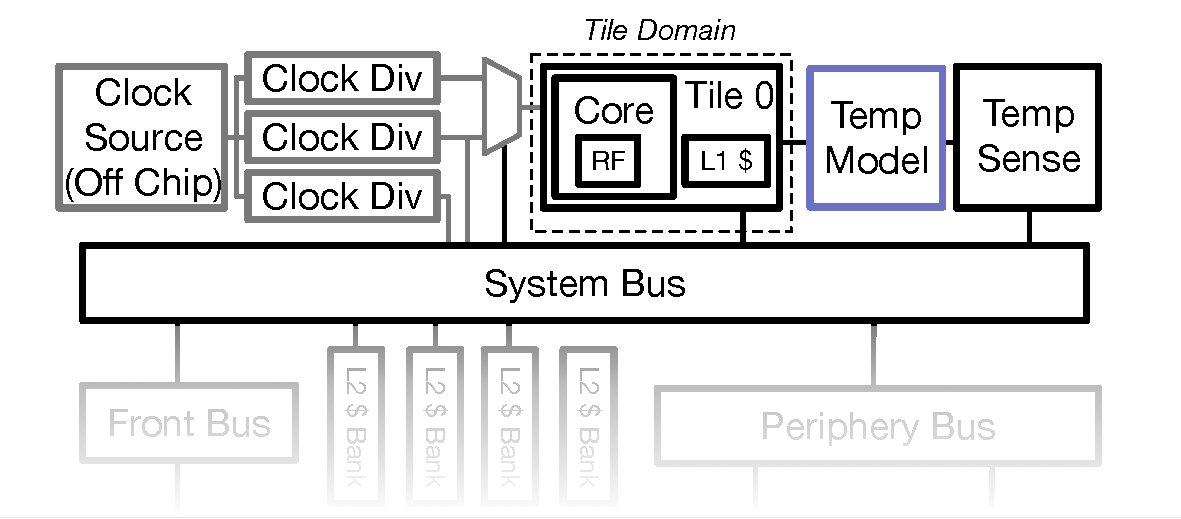
\includegraphics[width=0.99\textwidth]{figures/pdes-demo-target.pdf}
    % graffle2pdf -c pdes-demo-truncated midas-graphics/graffle/midas2-target.graffle figures/pdes-demo-target.pdf
    \caption{}
    \label{fig:pdes-demo-target}
\end{figure}

To integrate a temperature model, we added a temperature sensor that consists
of a 8-bit memory-mapped register fed by a CPU-hosted temperature bridge.
Target memory-mapped reads to this register return two times the current
temperature, in Celcius. The bridge periodically updates this register as a
function of both tile cycles elapsed and instructions retired. To do so, the
bridge driver polls the module every $P$ uncore cycles, measures a change in
cycle count ($\Delta C$) and instructions retired~($\Delta I$), calculates an
updated temperature~($T_{new}$), and writes temperature back to the bridge. The
model selects a core voltage by adding a scaling factor proportional to $\Delta
C$ to a base. In the overwhelming majority of cases, $V$ will be either be the
base voltage or $1.5\times$ it, as the tile is unlikely to undergo a frequency
change in any given polling interval. We give the complete model below:
\begin{equation}
\begin{split}
    V           & = 0.5 + \frac{\Delta C}{2P} \\
    E_{dynamic} & \propto \Delta I * V^2 \\
    E_{static}  & \propto \Delta C * V \\
    Q_{heating} & \propto E_{dynamic} + E_{static} \\
    Q_{cooling} & \propto P (T_{ambient} - T_{old}) \\
    T_{new}     & = T_{old} + Q_{heating} + Q_{cooling}
\end{split}
\end{equation}


This simple model, while completely insufficient for doing meaningful power
studies, suffices for creating regimes of high dynamic power utilization which
can then induce linux to switch between the two operating points.

\subsection{System Software}
Practically speaking, the most time consuming aspect of building this prototype
was writing system software, since we could not reuse code from an
existing chip. While linux provides many generic drivers that can be
configured entirely from the device tree, in the short term it was easier
primitive drivers tailored for our target. We wrote two new kernel modules:

\begin{itemize}
        % Linux version
\item A frequency scaling driver (extending \texttt{cpufreq\_driver} that binds to
linux's \texttt{cpufreq} subsystem. The target-specific component of this
driver supplies a table of two operating points and implements functions for
initialization, de-initialization, and frequency switching. The latter accepts an index
into the aforementioned table and writes to the tile clock multiplexor accordingly.

\item A thermal zone device driver that implements a function to read the
temperature, and defines polling intervals, temperature trip points and
trip types. This driver polls the temperature sensor every 100 ms, and
has a trip point set to 40C.

\end{itemize}

In total this consisted of roughly 200 lines of mostly boilerplate C code.
Interaction between these two drivers is fairly straightforward.  When linux
brings up the \texttt{cpufreq} subsystem during boot, it creates a new policy
backed by our custom driver. We use Linux's \texttt{ondemand} governor for this
policy, which picks the fastest available operating point unless the system is
idle. Later in boot, the thermal zone device for our temperature sensor
initalizes and binds itself as a cooling device to the \texttt{cpufreq} policy
above. When the thermal zone device reads a temperature above 40C trip point,
\texttt{cpufreq} will restrict the available operating points of the policy to
strictly the slower frequency. When this occurs the policy is then forced to
update: it switches the to the available operating point, which produces a
write to a memory-mapped register driving our clock mux. When the temperature
drops below this trip point, both operating points become available, and so,
unless the system is idle, the ondemand governor picks the faster operating
point and the clock mux setting is updated.

\subsection{Demonstration}

To demonstrate the operation of this system, we booted Linux on the target
above, with our custom drivers, and ran the SPEC 2017 benchmark
\texttt{641.leela} with its smaller ``test" input. In
Figure~\ref{fig:pdes-demo-plot}, we plot temperature~(C) and IPC versus time
(measured in uncore cycles). We calculate IPC in terms of the fixed uncore
clock, to better highlight operating point changes: this permits rocket's IPC
to reach two when running at the faster operating point.  Regions of the graph
shaded in lavender indicate the core is running at the slower operating point;
the graph has white background otherwise.

\begin{figure}
    \centering
    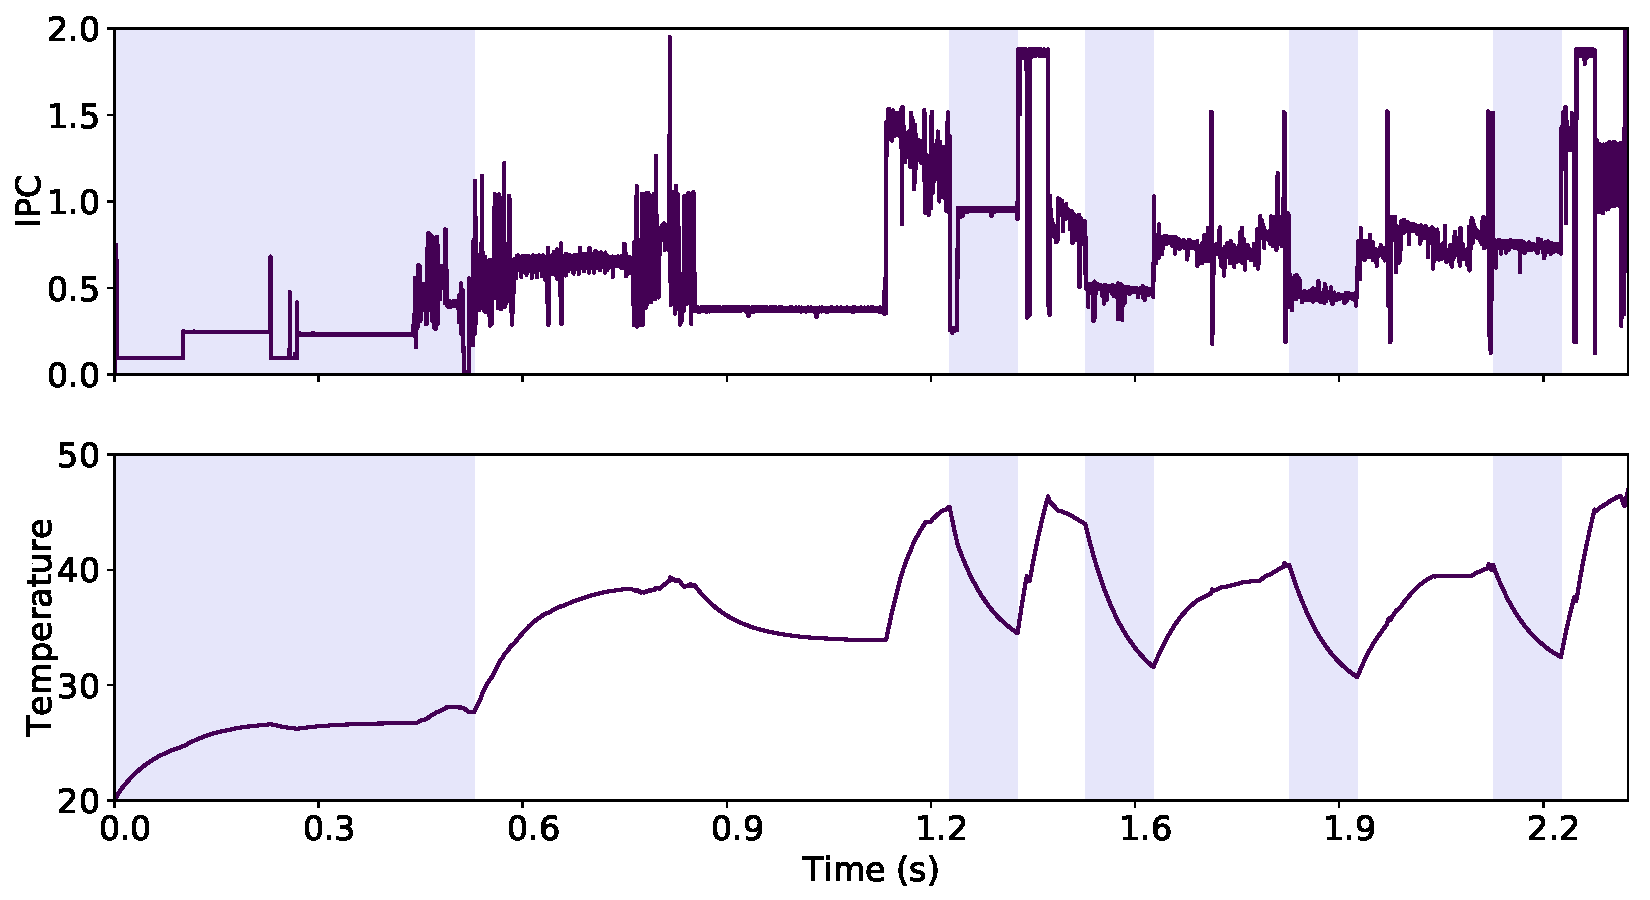
\includegraphics[width=0.99\textwidth]{figures/pdes-demo-plot.pdf}
    \caption{IPC and temperature (C) versus uncore cycle for \texttt{641.leela} running its 
    test input. Regions in lavendar indicate the core is running at the slower operating point (uncore frequency)
    whereas regions in white indicate is core is running at two times the uncore frequency.}
    \label{fig:pdes-demo-plot}
\end{figure}

After coming out of reset, the core is clocked at the slower frequency. It
remains at this frequency until linux brings up the \texttt{cpufreq} subsystem.
After initialization, the governor switches to the faster operating point.
Later during linux boot the thermal zone device for our temperature sensor is
registered, and bound to the \texttt{cpufreq} policy above. Since the device is
not above 40 C, no frequency changes are made immediately.

The first throttling event occurs around \TODO{}, after a relatively low IPC
period at the start of the benchmark. Here there is a precipitious drop in IPC
that reflects that the core frequency has been halved. After one polling
interval of the sensor, the temperature of the device has dropped sufficiently
to reenable the faster operating point, and the policy switches back to the
faster mode. The policy performs this dance for the remainder of the
simulation, though later periods of relatively lower IPC permit the device to
run at the higher frequency longer before the core is throttled.

We ran this workload on an earlier version of our prototype that used the
baseline TUs. We measured This configuration is  has Since this clock
organization configuration of this target matches the clock-mux configuration
of Figure~\ref{fig:clock-organizations} we'd expect an FMR of approximately
2.0, plus some additional bridge-induced slow downs if we were to rerun this
simulation with our optimized TUs.

\section{Interaction with Multi-Cycle Optimizations}

One justification for exploring the distributed approach described in this
chapter, was that a potential FMR increase may overlap with those brought about
by multi-cycle optimizations, hiding some or all of the potential slowdown. 
 In larger target systems, where multi-cycle
optimizations must be deployed, FMR can be signficantly higher because tokens
must propogate between a hub and spoke~(the same effect responsible for 2
cycles of latency in our clock gate organization), and the unit itself takes
multiple host cycles to process one target cycle.
As we explored in
Section~\ref{sec:pdes-common-circuit-perf} and
Section~\ref{sec:pdes-opt-units}, in some cases FMR will necessarily be larger
that the lower bound of two.

We leave more complete study of performance interactions to future work, as the
interactions brought about composing our distributed clock generation and
multicycle resource optimizations can quickly become complex. However, to
illustrate this effect we measure the performance of two quad-core BOOM
simulators, one based off mainline FireSim and one using the work of this
chapter. As we reported in original ICCAD paper~\cite{GoldenGate}, this system
cannot fit on the VU9P device provided by EC2 F1\footnote{Indeed, the
``LargeBoom" configuration has grown substantially since publication -- now
only a single core will fit on the FPGA without resource
optimizations\TODO{albert disseration}}, and so we will recruit the assistance
of the multi-cycle RAM optimization.  ote, the target RTL for these two systems
is indentical, except for clock generation.  Both of these systems have three
classes of clock domain, a 500 MHz DRAM domain, a 750 MHz uncore domain, and
1.5 GHz tile domains. The baseline system uses the clock generation scheme
described in the previous Chapter. Here all 4 cores staticlly clocked, and
essentially reside in the same domain.  For our PDES approach, we match what
was done in the thermal throttling demo. A high-speed clock source~(1.5 GHz)
feeds parallel clock dividers to provide the uncore and DRAM clocks, and each
of the four cores is given its own tile clock mux, this effectively puts each
tile in it's own clock domain. Resource utilziation is approximately the same
across the two designs, though the PDES configuration uses seven BUFGCEs over
the baseline of three.  We closed timing for both simulators at \TODO{40 MHz}.


\TODO{Discussion}

\section{Limitations and Future Work}\label{sec:pdes-future-work}

From the outset, the attractive aspect of our PDES-based approached, was that
it provided a flexible abstraction to inject arbitrary models of non-SSM
circuits. The cost of this abstraction is increased FMR. In some cases, latency
introduced by modelling timestamped units can be overlapped with the increased
execution time of multi-cycle models -- in this way, our approach dovetails
nicely with Golden Gate's defining feature.

However, the overwhelming majority of FireSim users simulate smaller target
systems in which no optimizations are required, and the expectation is that
simulators run close to unity FMR. So, for this approach to be viable, it needs to recoup the performance
losses it has introduced over the static case we described in the previous
chapter. Here are there two primary considerations, overcome throughput bounds
in feed-forward topologies, and overcome latency bounds intoduced in cycles of
the timestamped graph.

\subsection{Overcoming Throughput Bounds}
To replace the existing multi-clock implementation in FireSim, overcoming the throughput bounds of feed-forward networks
is sufficient, as networks of clock sources and clock-dividers are sufficient to reimplement the features of the clock bridge.

The best case FMR of our approach is currently two because positive and
negative edges for clocks are enqueued and dequeued as seperate messages. There
are a few potential fixes for this: the first is to use a better clock-message
encoding (e.g, one that encodes both positive and negative edge times), and
update TUs to act on these new tokens. This is not a panacea, because both
positive and negative edge times may not be known at enqueue time. In practise,
TUs would need to support both single and double-edged variants of clock
messages.  For fixed clocks whose frequencies are not statically defined, the
time zero message could simply encode the period and phase of the clock --
sinks would need only one message to be set for the remainder of simulation.
An alterative approach to keep TUs simple is to run parts of the timestamped
subgraph at two times $f_{fpga}$. Channels could then pack and unpack edges
into pairs, before presenting them to the hub.

The FMR-of-two limitation is a special case of a larger problem, the fastest
simulated clock in the system requires two host cycles to simulate each target
clock cycle. If the fastest clock in the system is not used to drive logic, but
is only fed into dividers to produce the clocks used by the system this cost
grows. In a system with clocks running at 1.5 GHz, 1 GHz, and 750 MHz~(as in
our system described in the previous Chapter), using only integer dividers
requires a 3 GHz reference clock (the LCM of the desired clock frequencies).
With the optimizations above, the system would run with FMR of two for the core
domain. To impove this, and support modelling high-frequency clock generators
like VCOs, a multi-period encoding of clocks is unavoidable.

Without this there are two simple paths forward. The first is to preclude
modelling high-frequency clock sources and downstream dividers as distinct
units, but instead fold them into a single unit.  This removes the high
frequency channel from the graph. Since output dividers are often integrated
into PLL IP, it would be natural to swap them out together and replace them
with a general but abstract PLL model whose implementation is optimized to
ensure high output message throughput. Alternatively, if we do not wish to
modify clock token encodings, clock dividers could be configured to assume
their inputs have fixed periods, this would permit them to look arbitrarily far
ahead of their inputs. Indeed, if constraints on the behavior of TUs could be
propagated across the graph of TUs at compile time, it would enable a variety
of global optimizations that could radically improve FMR -- this is relevant to

\subsection{Overcome latency bounds}
If there is a fundamental problem with the deadlock-avoiding approach we've
outlined in this chapter, it is latency though loops in the simulation graph can substiantially drive up
FMR. This is very evident in the baseline models, we implemented which require multiple null-message resolution cycles.
Even when null-message resolution is unnecessary, since many clocking
primitives are tightly coupled to the rest of the target (e.g., clock gates),
it not always possible to build TUs that have sufficient looakahead to
hide message transmission and hub-unit pipeline latency.

Staying within the regime of decoupled TUs, there are a few general approaches
to improving FMR.

Directly Cut latencies: The four-cycle update loop between the hub and a TU could be
improved by using flow-through queues between the hub-unit and sink TU, shaving
one cycle of latency. It may also be possible to remove a stage in the hub's
control pipeline, but this is highly dubious in targets with many timestamped
channels.

More intellegent channel implementation: Currently null-messages occupy slots
in the channel implementations, this may produce a form of head-of-line
blocking, where a TU is forced to dequeue a null message before being able to
observe a real transition, adding an extra cycle of latency. In practice there
is no need to enqueue null messages, instead, the channel could update a
secondary time register whose value would always match or exceed the timestamp
of the non-null message at the head of the queue. When any message would be
enqueued this value is increased. Null-messages could then be dropped with no loss of information.

\subsection{Alternative Approaches}




%\section{Deadlock Considerations}

%Patents:
%https://patents.google.com/patent/US20150046144A1/en
%
